\documentclass[border=10pt]{standalone}
\usepackage{tkz-euclide}

\begin{document}

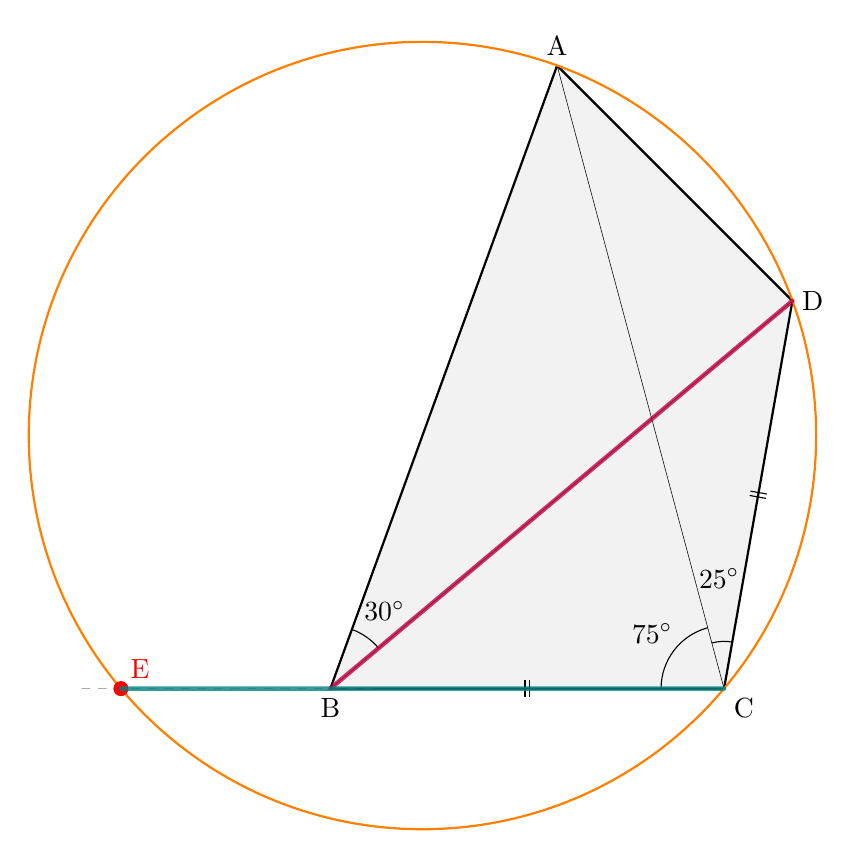
\begin{tikzpicture}
    
\tkzDefPoints{0/0/D,0/0/E,0/0/P2,0/0/O,0/0/A}
\tkzDefPoint(0,0){B}
\tkzDefPoint(5,0){C}

% Define B by rotating D around C by 100 degrees.
\tkzDefPointBy[rotation=center C angle -100](B) \tkzGetPoint{D}

% STEP 2: Find the location of point A using a compatible method.
% We define the two lines whose intersection is A.

% --- Define Line 1 (passing through C at a 25-degree angle to CD) ---
% We create a helper point 'P1' by rotating D around C. This is a reliable method.
\tkzDefPointBy[rotation=center C angle 25](D)  \tkzGetPoint{P1}

% --- Define Line 2 (passing through B at the correct angle) ---
% The absolute angle of the line segment BA should be 210 degrees.
% We create a helper point 'P2' on this line in a robust two-step way:
% 1. Define a point 'P_helper' at a 210-degree angle from the origin.
% 2. Create P2 by moving 'P_helper' by the same vector that goes from C to B.
\tkzDefPointBy[rotation=center B angle 30](D)
\tkzGetPoint{P2}

% --- Find A ---
% A is the intersection of the line (C, P1) and the line (B, P2).
\tkzInterLL(C,P1)(B,P2)
\tkzGetPoint{A}

% STEP 3: Draw the quadrilateral and its diagonals.
\tkzDrawPolygon[thick, fill=gray!10](A,B,C,D)
\tkzDrawSegment(A,C)
\tkzDrawSegment(B,D)

% STEP 4: Label the vertices.
\tkzLabelPoint[above](A){A}
\tkzLabelPoint[below](B){B}
\tkzLabelPoint[below right](C){C}
\tkzLabelPoint[right](D){D}

% STEP 5: Mark the given angles and equal sides.
\tkzMarkAngle[size=0.8, fill=blue!20,](D,B,A)
\tkzLabelAngle[pos=-1.2](A,B,D){$30^\circ$}
\tkzMarkAngle[size=0.8, fill=green!20](A,C,B)
\tkzLabelAngle[pos=-1.15](B,C,A){$75^\circ$}
\tkzMarkAngle[size=0.6, fill=red!20](D,C,A)
\tkzLabelAngle[pos=-1.4](A,C,D){$25^\circ$}
\tkzMarkSegment[mark=||, size=3pt](C,B)
\tkzMarkSegment[mark=||, size=3pt](C,D)

% STEP 6: Draw the circumcircle of triangle DAC.
\tkzDefCircle[circum](D,A,C)
\tkzGetPoint{O}
\tkzDrawCircle[color=orange, thick](O,A)

% % STEP 7: Extend line CB to find E on the circle.
\tkzInterLC(C,B)(O,A) \tkzGetPoints{E}{C_on}
\tkzDrawLine[color=gray, dashed](B,E)
\tkzDrawPoint[color=red, size=5pt, fill=red](E)
\tkzLabelPoint[above right, color=red](E){E}

% % STEP 8: Highlight the segments BD and CE for the proof.
\tkzDrawSegment[color=purple, ultra thick, opacity=0.8](B,D)
\tkzDrawSegment[color=teal, ultra thick, opacity=0.8](C,E)

\end{tikzpicture}


\end{document}